\section{GitHub Action}

A GitHub action is something that automatically happens when the status of a git repository changes on GitHub.
GitHub actions can be used to compile executables, run tests, deploy services, and do other automatic things.
This repository uses an action to compile a PDF!

We use an action called \texttt{latex-action}~\cite{latex-action} which uses a maximal TeXLive environment (meaning that most packages will already exist in the TeX installation).
If you need a non-standard LaTeX package, you can \texttt{apt-get} it---see the action's \href{https://github.com/dante-ev/latex-action/blob/master/README.md}{\texttt{README.md}} for details.

This action runs when code is \texttt{push}ed, or a branch is \texttt{pull\_request}ed.  You can adjust the events that trigger this action by changing the \texttt{on} setting of \href{https://github.com/evanberkowitz/latex-base/blob/gh-action/.github/workflows/main.yml}{.github/workflows/main.yml}.

To check that the PDF's source code is correct, this action attempts to compile it.  You can choose the compilation target by adjusting \texttt{jobs:env:target} from \texttt{master} to your preferred target, again in \href{https://github.com/evanberkowitz/latex-base/blob/gh-action/.github/workflows/main.yml}{.github/workflows/main.yml}.

This action produces an \emph{artifact}---something that survives after the automatic action is finished.
It creates a PDF that you can look at!

To see this PDF, you need to look at the checks of the commit (or pull request).
To find the details of the checks, find the symbol next to the commit---it might be a red X (indicating a failure), a yellow dot (indicating that the action is in progress), or a green check (indicating the action succeeded).
Click that symbol and then click `details', as suggested in the screenshot below.
\begin{center}
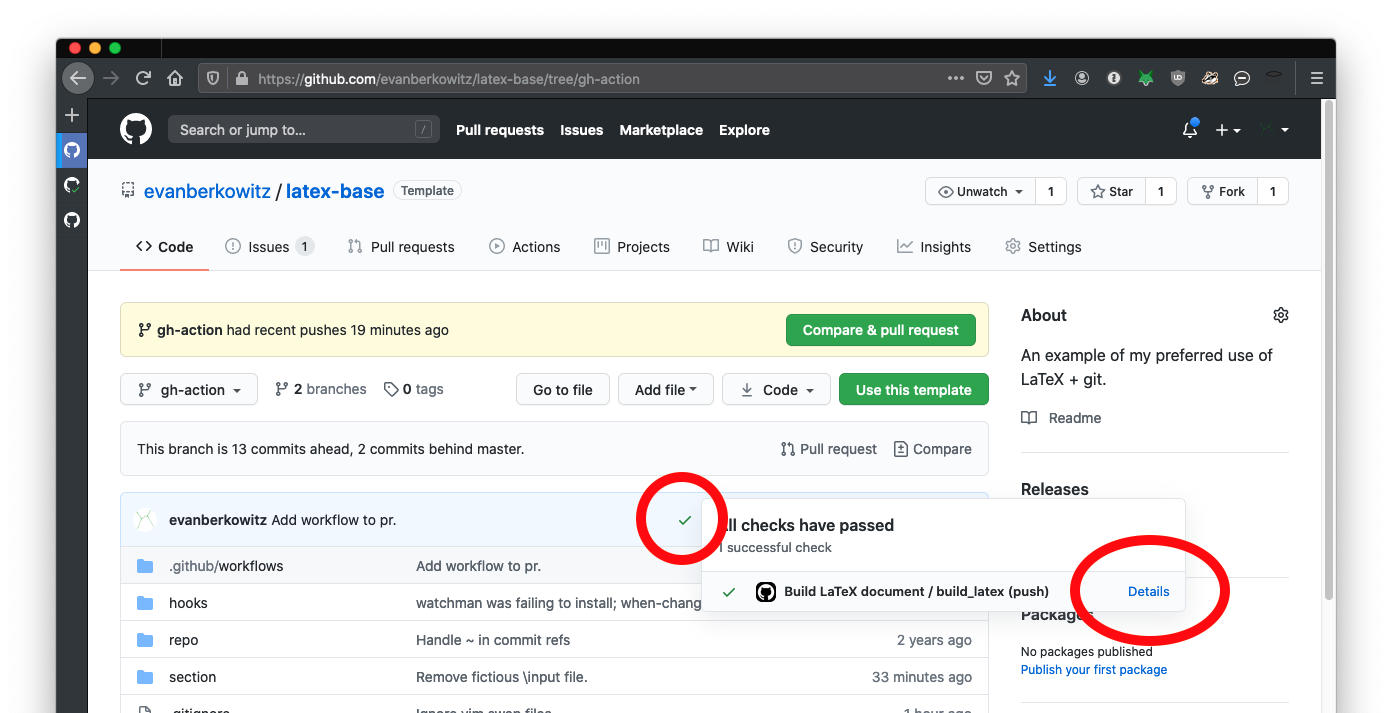
\includegraphics[width=0.75\textwidth]{figure/github-action-find-details}
\end{center}
To see the PDF, one must download the artifact, as shown in the screenshot below.
Artifacts are named after the target, and are suffixed with the SHA of the commit.
Artifacts are always ZIP files.  When you unzip it you will see a PDF, which reflects the state of the code after that commit.
\begin{center}
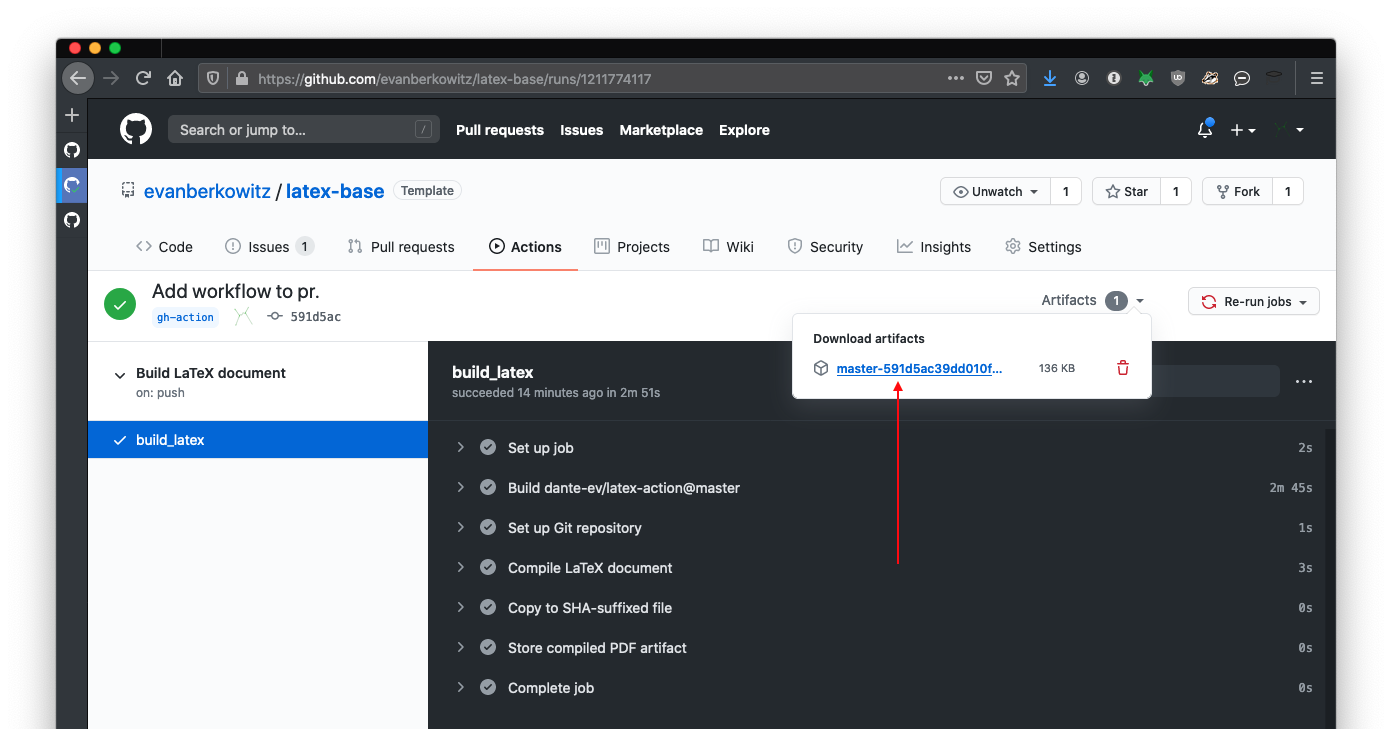
\includegraphics[width=0.75\textwidth]{figure/github-action-artifact}
\end{center}
To turn off the repository information printed on the side of the PDF, add \texttt{FINAL=1} to the \texttt{args} of the \texttt{latex-action} step of the \href{https://github.com/evanberkowitz/latex-base/blob/gh-action/.github/workflows/main.yml}{.github/workflows/main.yml}.


